\chapter*{Summary\footnote{This chapter incorporates abstracts, discussions, and conclusions from several publications.}\markboth{Summary}{}}
\addcontentsline{toc}{chapter}{Summary}

Nowadays, lifelong learners learn in scattered moments throughout the day and the week, and they have to balance learning activities with work, family and leisure schedules. In this thesis, we started by getting grasp of how, when, what, and where do lifelong learners learn using their mobile devices as a key channel to support them across contexts. Therefore, chapter 1 highlighted these patterns as a starting point to understand how lifelong learners learn and to identify in which contexts lifelong learners might need support. 

\begin{figure}
     \centering
     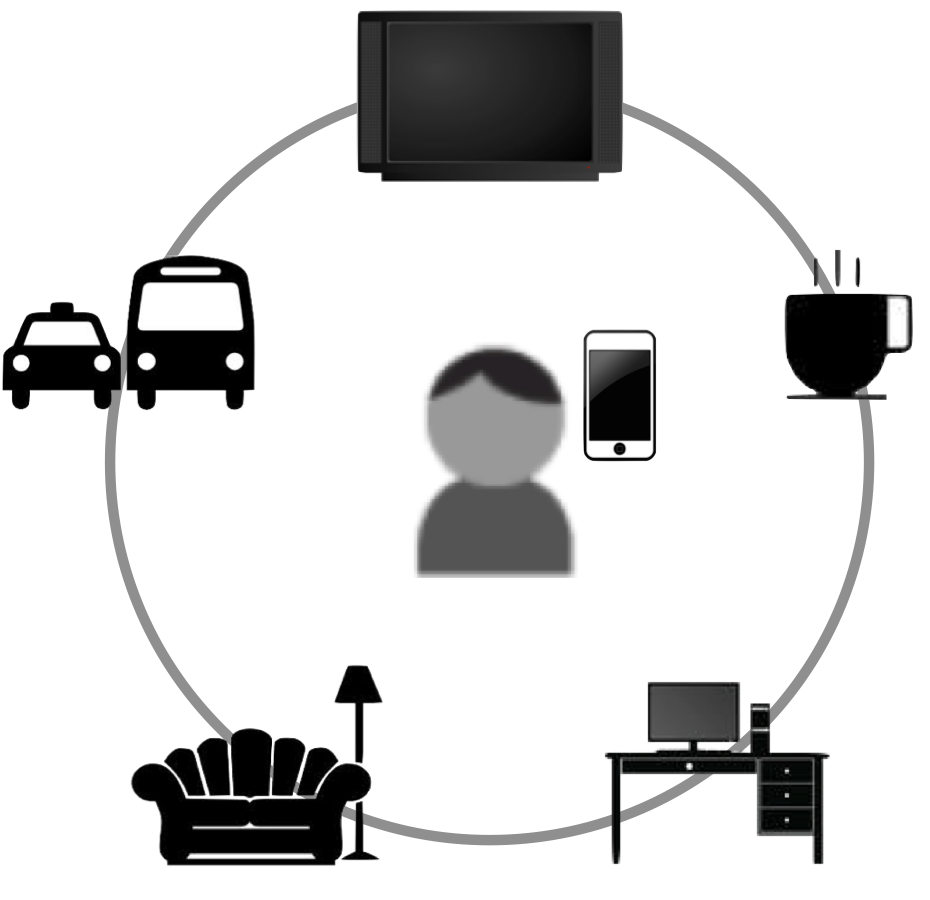
\includegraphics[width=0.5\linewidth]{img/summary_fig1}
     \caption{Lifelong learners' available resources}
     \label{fig:summary_1}
\end{figure}

In this thesis, the smartphone is identified as the most able partner \citep{Luckin2008} to support lifelong learners across contexts (figure \ref{fig:summary_1}:  e.g. at home, at work, commuting, having a break) since it is always carried around with the learner. Indeed, the smartphone represents a 24-hours a day and 7-days a week available access channel to existing educational resources hosted in the cloud, as well as powerful tool to author new educational resources. Offering educational resources openly is one of the key policies to facilitate universal access for lifelong learners. Thus, in chapter 2 we have observed the current support from content repositories to mobile devices, identifying best practices and suitable architectures for the implementation of software that might facilitate universal access to content stored in repositories. Additionally, smartphones enable learners to author educational resources not only providing channels to share, remix or re-contextualize these, but also capturing the context in-situ and in-time. As a further matter, authoring educational resources in a mobile context is an authentic experience where authors can inspire learning resources on their own daily life activities and reflections. Thus, chapter 5 exposed a literature review of mobile authoring tools, in which 10 limitations obstructing mobile authoring of OER were identified. Based on these findings, a mobile authoring tool of OER covering most of these limitations was implemented, evaluated, and the code shared under open source for further developments.

\begin{figure}[ht]
  \begin{adjustbox}{
  	addcode={
  		\begin{minipage}{\width}}{
	  		\caption{Classification framework for sampling experiences on mobile devices}
		\end{minipage}},rotate=90,center}
      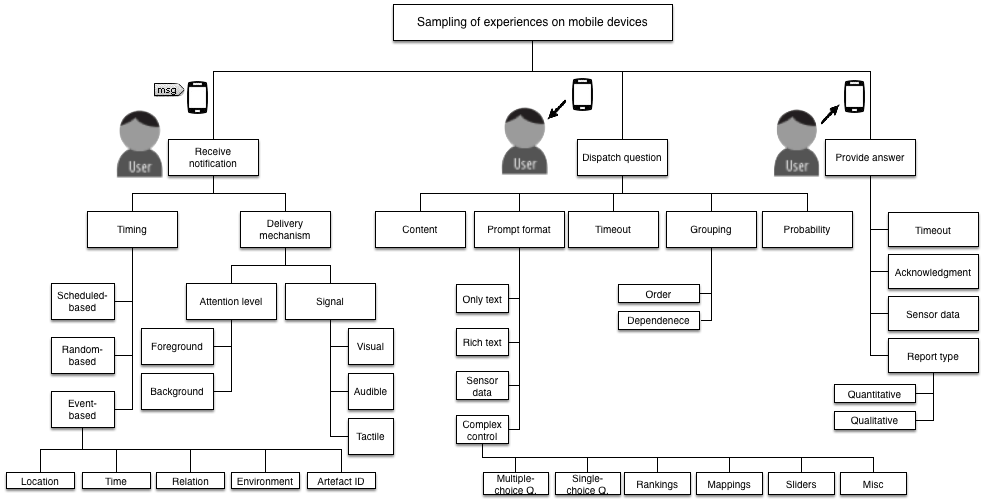
\includegraphics[scale=.6]{img/Esm_fig1}
      \label{fig:summary_2}
  \end{adjustbox}
\end{figure}

A strength of lifelong learners is their intrinsic motivation to study and their continuous career development. Hence, they continuously try to understand the way they learn, avoiding obstacles (i.e. time, location, technology), and scaffolding learning activities in daily physical environments. In this thesis, we proposed lifelong learners to introspect their learning habits reporting their reflections on mobile devices as key benchmarks to become aware of successful learning environments and to identify personal learning preferences in context (i.e. preferred time, location, resources). Therefore, a classification framework for sampling of experiences on mobile devices is presented (See figure \ref{fig:summary_2}) and piloted in chapter 4. Later on, this framework is deeper instantiated in experimental settings (chapters 6, 8, 9). 

In chapter 6 we identified the lack of support for learning activities across locations, devices, and environments, as well as, the necessity to link learning activities with everyday life activities as key challenges for lifelong learners. There is very little research on how to link the different everyday contexts of lifelong learners and their learning activities in these different settings. Thus, based on the literature review presented in chapter 3, the implementation of a mobile tool with low-complexity interactions (NFC based) is proposed as a suitable approach to provide seamless support for lifelong learners in the task track their time devoted to learn across locations, devices and environments. As reported in chapter 1, lifelong learners recur to certain physical spaces (e.g. sofa, desktop) or moments (e.g. commercial breaks on TV, waiting times, commuting) to accomplish their learning activities. The NFC-LearnTracker presented in this thesis was recognized as a relevant tool with the potential identify those successful learning environments, to manage self-defined learning goals, to keep track of the time devoted to each learning goal, and to monitor their progress with learning analytics visualizations.

In this thesis we aimed at supporting learners to understand the way they can better learn using technology, therefore we focused on two specific key competences for lifelong learning \citep{EuropeanCommission2007}, namely,  \em learning to learn \em and  \em digital competence \em.

On the one hand side, learning to learn implies the learner to understand how to make the best use of own skills and available resources towards the accomplishment of self-defined learning goals. In chapter 8, we instantiate again the classification framework for sampling experiences (see figure \ref{fig:summary_2}) by prompting learners compact and structured notifications suggesting to examine and evaluate their own learning. These notifications were prompted as structured and repeated introspective episodes, offered during the course of the learning action as well as after the learning action, to make learning visible. The results show that students do not have a habit to see themselves as learners and to develop a "professional" awareness about their daily activity at work/school. 

The effectiveness of mobile notifications to foster reflective practice on meta-learning is further researched in the longitudinal study from chapter 9. Observing at the timing when the notification were offered, the findings conclude that notifications pushed at random time of the day do not produce significant improvements in time management. Nevertheless, notifications pushed at fixed times of the day moderate positively the measure of time management. These results are consistent with the answers reported by the learners regarding their timing preference in which, notifications at 10h were preferred over notifications at 20h as well as over notifications randomized in time. Another reason to argue on these results might be that students prefer notifications that persuade them to (pre-)�plan ahead� their learning day, rather than (post-)�look backward� their learning day or (in-action) �plan� at any moment of the day. Observing at the content of the notifications, the findings in the experiment suggest that notifications containing learning analytics and tips for self-regulation influence positively the skill of time management. More specifically, notifications containing learning analytics resulted in slightly higher scores. Likewise, chapter 9 provides an interesting perspective on how learners devote their time to learn throughout the day, along the week and in long term.

On the other hand, digital competence involves the confident and critical use of technology to learn, work, and communicate in personal and social life. Nowadays, technology is constantly shaping the way we learn, thus designing interfaces that are easy to use and to integrate into daily life activity becomes increasingly relevant for lifelong learners. This assumption is reinforced by the results reported in the second study from chapter 8, in which the group assigned with the least complex interactions on mobile devices envisioned higher knowledge and motivation scores. Likewise, ours assumptions are strengthen by the measures of complexity, the usability test, and the observations of participation presented in the experiment from chapter 9.

The results from the survey in chapter 1 show that lifelong learners reported their living room (and sitting in the sofa) as the most suitable environment to watch videos using their mobile devices for learning purposes. In chapter 3, we orchestrate an ecology of digital resources in the context of this specific environment to facilitate casting of video content stored in the cloud by lowering the complexity of interactions with devices (i.e. reducing the time to start the learning activity, reducing the number of clicks to access the learning content), as well as improving the resolution casting HD quality as an alternative to small-sized definition on mobiles, tablet or laptops. 

In this research, we investigated different ways to foster the competence of �learning to learn�, using SMSs and mobile chart visualizations as channels to provide guidance (external feedback). The differentiation among external and internal feedback is crucial if one investigates the effects of feedback viewing the process of knowledge acquisition as a self-regulated learning process \citep{Narciss2007}. Hence, we will extend this research scaffolding ecologies in which lifelong learners are able to customize internal feedback based on their own occasional learning priorities and contingencies.


